\documentclass[12pt]{article}
\usepackage[a4paper, margin=.30in]{geometry}
\usepackage{graphicx ,
            wrapfig,
            xcolor, 
            enumerate,
            amsmath,fontenc, mhchem  ,tcolorbox, chemfig, makecell
            }
\usepackage{multirow}
\newcommand\headerMe[2]{\noindent{}#1\hfill#2}
\renewcommand{\thesection}{\Roman{section}}

\author{Zakaria HAOUZAN}
\date{\today}

\begin{document}
% headers --------------
\headerMe{Matière : Physique-Chimie}{Professeur : Zakaria HAOUZAN}\\
\headerMe{Unité : Travail Mécanique et Energie }{Établissement : Lycée SKHOR qualifiant}\\
\headerMe{Niveau : 1BAC-SM-X}{Heure : 7H}\\

% ------Content ________
\begin{center}

  \Large{Leçon $N^{\circ} 9 $: \color{red} Molécules organiques et Modification du squelette carboné  }
\end{center}

%\begin{wrapfigure}[10]{r}{0.5\textwidth}
%    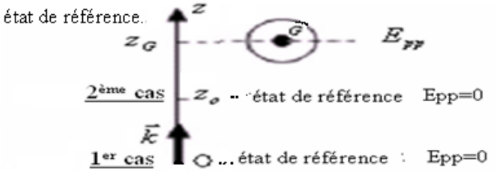
\includegraphics[width=0.5\textwidth]{./img/img00.png}
%\end{wrapfigure}


%\begin{tcolorbox}[colback=pink!10!white,
                  %colframe=blue!15!gray,
                  %title=Application -1- :
                 %]


  %\begin{wrapfigure}[10]{r}{0.3\textwidth}
  %\vspace{-2cm}
    %\includegraphics[width=0.3\textwidth]{./img/Mode_opératoire_dosage:.png}
%\end{wrapfigure}


\section{Les alcanes :}
  \subsection{ Définition des alcanes: }
Les alcanes sont des hydrocarbures saturés (ils sont constitués par des atomes de carbone et des atomes d'hydrogène liés entre eux par des liaisons simples C-C et C-H).

  La formule brute générale des alcanes est : $C_nH_{2n+2}$ ( n : entier naturel non nul).

\begin{tcolorbox}[colback=pink!10!white,
                  colframe=blue!15!gray,
                  title=Remarque  -1- :
                 ]
  \textbf{La formule brute :} indique le nombre et la nature des atomes constituant la molécule.

  \textbf{la formule développée: }fait apparaître tous les atomes et toutes les liaisons entre les atomes de la molécule.

  \textbf{La formule semi-développée: }fait apparaître tous les atomes et toutes les liaisons entre les atomes à l'exception des
liaisons avec les atomes d'hydrogène.

  \textbf{La formule topologique:} est une représentation simplifiée dans laquelle la liaison entre les atomes de carbones est représentée par un segment dont chaque extrémité correspond à un atome de carbone.

\end{tcolorbox}
Exemple : le propane
  \begin{center}
    \begin{tabular}{ |c|c|c|c| } 
\hline
      formule brute & formule plane développée & formule semi-développée& représentation topologique \\
\hline
      $\ce{C_3H_8}$& \chemfig{H-C(-[6]H)(-[2]H)-C(-[6]H)(-[2]H)-C(-[6]H)(-[2]H)-H}&$\ce{CH_3-CH_2-CH_3}$&\chemfig{[1]-[-1]-}\\\hline
      \hline
\end{tabular}
  \end{center}



  \section{ Nomenclature des alcanes:}
  \subsection{Cas des alcanes à chaine linéaire:  }

Le nom d'un alcane est formé d’un terme dépendant du nombre d’atomes de carbone dans la chaîne, suivi du suffixe “ane”
  \begin{center}
    \begin{tabular}{ |c|c|c|c|c| } 
\hline
      \makecell{Nombre \\d'atome \\de Carbone} & \makecell{formule\\ brute} & \makecell{Nom de\\ l'alcane}& Sa formule semi-développée& \makecell{Ecriture \\topologique}\\
\hline
      1 &$\ce{CH_4}$    & méthane& $\ce{CH_4}$ &  x\\\hline
      
      2 &$\ce{C_2H_6}$  & éthane& $\ce{CH_3-CH_3}$ &  $\ce{-}$\\\hline
      
      3 &$\ce{C_3H_8}$    &propane & $\ce{CH_3-CH_2-CH_3}$ & \chemfig{[1]-[-1]-} \\\hline
                                                                         % -[1]-[-1]-[1]-[-1]
      4 &$\ce{C_4H_{10}}$ &butane& $\ce{CH_3-CH_2-CH_2-CH_3}$ & \chemfig{-[1]-[-1]-[1] } \\\hline
      
      5 &$\ce{C_5H_{12}}$ &pentane& $\ce{CH_3-CH_2-CH_2-CH_2-CH_3}$ & \chemfig{-[1]-[-1]-[1]-[-1] } \\\hline
      
      6 &$\ce{C_6H_{14}}$ &hexane& $\ce{CH_3-CH_2-CH_2-CH_2-CH_2-CH_3}$ & \chemfig{-[1]-[-1]-[1]-[-1]-[1] } \\\hline
      \hline
\end{tabular}
  \end{center}
  
  \begin{center}
    \begin{tabular}{ |c|c|c|c|c| } 
\hline
      \makecell{Nombre \\d'atome \\de Carbone} & \makecell{formule\\ brute} & \makecell{Nom de\\ l'alcane}& Sa formule semi-développée& \makecell{Ecriture \\topologique}\\
\hline
      
      7 &$\ce{C_7H_{16}}$ &heptane& $\ce{CH_3-CH_2-CH_2-CH_2-CH_2-CH_2-CH_3}$ & \chemfig[angle increment=77]{-[1]-[-1]-[1]-[-1]-[1]-[-1] } \\\hline
      
      8 &$\ce{C_8H_{18}}$ &octane& $\ce{CH_3-CH_2-CH_2-CH_2-CH_2-CH_2-CH_2-CH_3}$ & \chemfig[angle increment=77]{-[1]-[-1]-[1]-[-1]-[1]-[-1]-[1] } \\\hline
      
      9 &$\ce{C_9H_{20}}$ &nonane& $\ce{CH_3-CH_2-CH_2-CH_2-CH_2-CH_2-CH_2-CH_2-CH_3}$ & \chemfig[angle increment=79]{-[1]-[-1]-[1]-[-1]-[1]-[-1]-[1]-[-1] } \\\hline
      
      10 &$\ce{C_{10}H_{22}}$ &décane& $\ce{CH_3-CH_2-CH_2-CH_2-CH_2-CH_2-CH_2-CH_2-CH_2-CH_3}$ & \chemfig[angle increment=80]{-[1]-[-1]-[1]-[-1]-[1]-[-1]-[1]-[-1]-[1] } \\\hline
      \hline
\end{tabular}
  \end{center}

\begin{tcolorbox}[colback=pink!10!white,
                  colframe=blue!15!gray,
                  title=Remarque  -2- :
                 ]
  Les radicaux alkyls ont pour formule brute $\ce{-C_nH_{2n+1}}$\\
  Le nom d'un radical alkyl s'obtient à partir du nom de l'alcane correspondent (qui a le meme nombre d'atomes de carbones) en échangeant la terminaison (ane) par (yle).
\end{tcolorbox}

\begin{center}
    \begin{tabular}{ |c|c|c|c|c| } 
\hline
      \makecell{Nombre \\d'atome \\de Carbone} & \makecell{formule\\ brute \\ de L'alcane} & \makecell{Nom de\\ l'alcane}&\makecell{L'alkyl \\correspondant} & \makecell{Son nom}\\
\hline
      1 &$\ce{CH_4}$    & méthane& $\ce{-CH_4}$ &  méthyle\\\hline
      
      2 &$\ce{C_2H_6}$  & éthane& $\ce{-C_2H_5}$ &  éthyle\\\hline
      
      3 &$\ce{C_3H_8}$    &propane & $\ce{-C_3H_7}$ & propyle \\\hline
                                                                         % -[1]-[-1]-[1]-[-1]
      4 &$\ce{C_4H_{10}}$ &butane& $\ce{-C_4H_9}$ &  butyle \\\hline
      
      \hline
\end{tabular}
  \end{center}
  


  \subsection{Nomenclature des alcanes ramifiés: }
  Le nom principal de l'alcane ramifié est donné par la chaine carbonée la plus longue devant lequel on place les nom des radicaux alkyl numérotés en utilisant les plus petits nombres possibles et classés par ordre alphabétique.

\begin{tcolorbox}[colback=pink!10!white,
                  colframe=blue!15!gray,
                  title=Remarque  -3- :
                 ]
Lorsque les mêmes radicaux sont répétés on utilise les préfixes multiplicateur ( mono, di , tri , tétra , penta
hexa , hepta ....) pour indiquer leur nombre.
  \end{tcolorbox}
Exemples:

  \begin{center}
    \begin{tabular}{ |c|c|c| } 
\hline
      \makecell{Alcane ramifié } & \makecell{Son Nom } & \makecell{Sa formule \\topologique}\\
\hline
      
      $\chemfig{CH_3-CH(-[6]CH_3)-CH_2-CH_3}$ & 2-méthyle butane &  \chemfig{-[1](-[2])-[-1]-[1]-[-1] }  \\\hline
      
      $\chemfig{CH_3-C(-[6]CH_3)(-[2]CH_3)-CH_2-CH_3}$ & 2,2 diméthyle butane &  \chemfig{-[1](-[2])(-[-2.5])-[-1]-[1]-[-1] }  \\\hline

      $\chemfig{CH_3-CH(-[6]CH_3)-CH_2(-[2]CH_3)-CH_2-CH_3}$ & 2,3 diméthyle pentane &  \chemfig{-[1](-[2])-[-1](-[-2])-[1]-[-1] }  \\\hline
      
      $\chemfig{CH_3-CH(-[6]CH_3)-CH(-[2]C_2H_5)-CH_2-CH_3}$ & \makecell{3-éthyle \\2-méthyle pentane }&  \chemfig{-[1](-[2])-[-1](-[-2](-[5]))-[1]-[-1] }  \\\hline
      
      $\chemfig{CH_3-CH(-[6]CH_3)-C(-[2]CH_3)(-[-2]CH_3)-CH_2-CH(-[2]C_2H_5)-CH_2-CH_3}$ & \makecell{5-éthyle \\2,3,3-triméthyle heptane} &  \chemfig[angle increment=55]{-[1](-[2])-[-1](-[-2])(-[1.5])-[1]-[-1](-[5](-[5.5]))-[1]-[-1] }  \\\hline

      $\chemfig{CH_3-CH(-[6]CH_3)-CH(-[2]CH_3)-C(-[2]CH_3)(-[6]CH_4)-CH_2-CH_3}$ & \makecell{2,3,4,4 tétraméthyle\\ hexane} &  \chemfig[angle increment=55]{-[1]-[-1](-[4.9])-[1](-[2])-[-1](-[5])(-[5.5])-[1]-[-1] }  
      \\\hline
                     
           \hline
\end{tabular}
  \end{center}

\subsection{Les cycloalcanes: }
Les cycloalcanes sont des hydrocarbures cycliques saturés dont la formule brute générale est : $C_nH_{2n}$ avec $n \geq3$

Le nom d'un cycloalcane s'obtient en utilisant le préfixe ''cyclo'' suivi par le nom de l'alcane correspondant.

Exemples:

\begin{center}
    \begin{tabular}{ |c|c|c| } 
\hline
      \makecell{ cycloalcane  } & \makecell{Son Nom } & \makecell{Sa formule \\topologique}\\
\hline
      
      $\chemfig{H_2C(-[1.5]CH_2?)-CH_2?}$ &cyclopropane &  \chemfig{?-[1]-[-1]-[4]? }  \\\hline 
      
      $\chemfig{H_2C(-[2]CH_2(-[0]CH_2?))-CH_2?}$ & cyclobutane &  \chemfig{?-[0]-[2]-[4]? }  \\\hline 
      
      $\chemfig{H_2C(-[2]CH_2(-[1.5]CH_2(-[-1.5]CH_2?)))-CH_2?}$ &cyclopentane &  \chemfig{?-[0]-[2]-[2.6]-[5.2]? }  \\\hline 
      
      $\chemfig{CH_2*6(-CH_2-CH_2-CH_2-CH_2-CH_2-)}$ &cyclohexane &  \chemfig{*6(------)}  \\\hline 

      $\chemfig{H_2C(-[1.5]CH_2?(-[3.5]CH_3))-CH_2?}$ &méthyle cyclopropane &  \chemfig{?-[1](-[3.5])-[-1]-[4]? }  \\\hline 
      
      $\chemfig{H_2C(-[1.5]CH_2?(-[2.5]CH_3)(-[1.5]CH_3))-CH_2?}$ &1,1-diméthyle cyclopropane &  \chemfig{?-[1](-[2.5])(-[1.5])-[-1]-[4]? }  \\\hline 
           \hline
\end{tabular}
  \end{center}

  \subsection{Les halogénoalcanes:}
Un halogénoalcane est un composé organique saturé qui possède (au moins) un atome d’halogène noté X : F pour fluor, Cl pour chlore, Br pour brome et I pour iode.
La nom de l' halogénoalcane s'obtient en utilisant le préfixe "fluoro, chloro, bromo ou iodo" suivi par le nom de
l'alcane correspondant.

Exemples:

\begin{center}
    \begin{tabular}{ |c|c|c| } 
\hline
      \makecell{1,2 dibromopropane } & \makecell{2-chloro butane} & \makecell{2-chloro 3-méthyle pentane}\\
\hline
      
      \makecell{ $\chemfig{CH_3-CH(-[6]Br)-CH_2-[6]Br}$\\
      \chemfig{-[1](-[2]Br)-[-1]-[6]}
      } &
      \makecell{$\chemfig{CH_3-CH_2-CH(-[6]Cl)-CH_3}$\\ $\chemfig{-[1]-[-1](-[6]Cl)-[1]}$}
      &  $\chemfig{CH_3-CH(-[6]Cl)-CH(-[6]CH_3)-CH_2-CH_3}$  \\\hline 
                \hline
\end{tabular}
  \end{center}

\subsection{Les isomères:}
Les molécules qui ont la même formule brute mais ont des formules développées différentes s'appelles des isomères.
Dans le cas des alcanes on distingue deux types d'isomérie :
\begin{itemize}
  \item -L'isomérie de position :ils ont la même formule brute mais de position différente\\ 1-chlorobutane : $\chemfig{CH_3-CH_2-CH_2-CH_2-[6]Cl}$ et 2-chlorobutane :  $\chemfig{CH_3-CH_2-CH_2(-[6]Cl)-CH_2}$
  \item L'isomérie de chaine : sont des isomères de chaine ils différent par leur chaine ils ont la même formule brute.\\Exemple 2,2-diméthyle propane et 2-méthyle butane et pentane
\end{itemize}
\subsection{Propriétés physique des alcanes:}
Les alcanes se présentent à température ambiante soit sous forme gazeuse (méthane, éthane, propane et butane), soit
sous forme liquide ( composés ayant entre 5 et 16 carbones) soit solide ( plus de 16 carbones). Ils sont insolubles dans
l'eau mais solubles dans la plupart des solvants organiques. Ce sont composés saturés stables et peu réactifs ils sont
chimiquement stables.

\section{Les alcènes :}
\subsection{Définition }
Les alcènes sont des hydrocarbures insaturés caractérisés par la présence d'une double liaison C=C .Leur formule brute  générale est $C_nH_{2n}$ avec $n\geq2$ entier naturel.
\subsection{Nomenclature des alcènes: }
La nomenclature des alcènes ressemble à celle des alcanes de même squelette, en remplaçant la terminaison " ane " par " ène". Dans ce cas la chaîne principale est la chaîne la plus longue qui contient la double liaison .

Remarque : On place entre deux tirets, le numéro (le plus petit possible) qui désigne la position de la liaison double.

Exemples: 

2- méthyle prop-1-ène : $\chemfig{CH_3-C(-[6]CH_3)=CH_2}$ :\hspace{1cm} $\chemfig{-[1](-[2])=[-1]}$

La stéréoisomérie (appelée aussi isomérie structurale) : dans ce type d’isomérie, les molécules ont la même formule brute, la même formule semi développée mais les substituants ont des configurations spatiales différentes.

\subsection{Isomérie:}
On dit que des molécules sont des isomères si elles possèdent la même formule brute et que leurs formules développées sont différentes.

On distingue chez les alcènes trois types d'isomères:
\begin{itemize}
  \item les isomères de position qui diffèrent par la bbposition de la double liaison .
    \\Exemple  : but-1-ène$CH_2=CH-CH_2-CH_3$ et $CH_2-CH=CH_2-CH_3$ but-2-ène
  \item - les isomères l'isomérie de chaîne : qui diffèrent par la structure de la chaîne des carbone.
  \item les isomères l'isomérie Z-E (ou cis-trans) :
    Il s’agit d’un cas particulier d’isomérie possible dans une molécule comportant une double liaison entre les deux
carbones liés à des atomes ou groupes chimiques différents.
\\Pour qu’une isomérisation Z ou E puisse avoir lieu, il faut remplir deux conditions :
\\la molécule doit présenter une double liaison carbone-carbone.
\\les groupes de part et d’autre de la double liaison doivent être différents.

Si les deux groupes les plus importants sont du même coté de la double liaison C=C alors l’isomère est de type Z.
(Zusammen qui veut dire ensemble en allemand).
Si les groupes prioritaires se trouvent de part et d’autre, il s’agit d’un isomère de type E .

    \end{itemize}
  %\begin{wrapfigure}[10]{r}{0.1\textwidth}
  %%\vspace{-2cm}
    %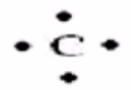
\includegraphics[width=0.1\textwidth]{./img/carbone_foem.png}
%\end{wrapfigure}

%  \section{ L'élément de base de la chimie organique : (Le Carbone)}
  



\subsection{Test d'identification des alcènes;}
On test la présence d'un alcène par l'eau de brome qui perd sa coloration orange en présence de l'alcène

\section{Modification des squelettes carbonées :}
\subsection{Craquage:}
Le craquage permet de transformer une molécule d'hydrocarbure en molécules plus courtes.
\\Exemple : craquage de l'octane .-craquage catalytique
\subsection{Reformage catalytique: }
Le reformage est un procédé industriel qui s'applique aux hydrocarbures en présence de catalyseurs à chaud et sous pression élevé, elle permet de modifier profondément la structure des hydrocarbures. On distingue trois types de
reformage : la cyclisation , la ramification et la déshydrogénation.

-La ramification :
Un alcane à chaine linéaire se transformer en un isomère à chaine ramifiée.

-La cyclisation :
A partir d'un alcane linéaire on obtient un alcane cyclique avec formation du dihydrogène.

-La déshydrogénation:
Elle consista à transformer une liaison covalente simple C-C en une liaison double C=C .

\end{document}

